\documentclass[11pt,letterpaper,titlepage]{article}
\usepackage{fancyhdr}
\usepackage[left=0.75in, right=0.75in, bottom=1.0in]{geometry}
\usepackage{lastpage}
\usepackage{titleref}
\usepackage{booktabs}
\usepackage{appendix}
\appendixtitleon
\appendixtitletocon

\makeatletter

%================== List of figures and tables mods
\usepackage{tocloft}
\usepackage[labelfont=bf]{caption}

\renewcommand{\cftfigpresnum}{Figure\ }
\renewcommand{\cfttabpresnum}{Table\ }

\newlength{\mylenf}
\settowidth{\mylenf}{\cftfigpresnum}
\setlength{\cftfignumwidth}{\dimexpr\mylenf+1.5em}
\setlength{\cfttabnumwidth}{\dimexpr\mylenf+1.5em}



%=================== Graphics
\usepackage{graphicx}
\usepackage[breakwords]{truncate}
\usepackage{float}
\usepackage{array}
\usepackage{amsmath}
\usepackage{mdframed}
\usepackage{fancyvrb}
\usepackage{float}
\usepackage{cancel}
\usepackage{amssymb}
\graphicspath{ {images/} }
\usepackage[usenames,dvipsnames,svgnames,table]{xcolor}
\usepackage[defaultlines=2,all]{nowidow}
\usepackage{listings}
\usepackage{color}
\definecolor{Brown}{cmyk}{0,0.81,1,0.60}
\definecolor{OliveGreen}{cmyk}{0.64,0,0.95,0.40}
\definecolor{CadetBlue}{cmyk}{0.62,0.57,0.23,0}
\usepackage{pdflscape}
\usepackage{relsize}
\usepackage{verbatim}
\usepackage{tabto}


%=================== Settings
\renewcommand{\baselinestretch}{1.2}
\definecolor{gray}{rgb}{0.4 0.4 0.4}
\newcommand{\stimes}{{\times}}

\begin{document}
\newcommand{\NSCDOCNUMBR}{NSC-REP-15-X}         %Put document number here
\newcommand{\NSCDOCSUBJT}{TECHNICAL REPORT: }   %Put document subject here
\newcommand{\NSCDOCTITLE}{$FALCON$ - Interfacing with Falcon BMS 4.33.3 $\chi -Tech$}       %Put document title here
\newcommand{\NSCDOCDATE} {May, 2017}    %Put document date here
\newcommand{\NSCDOCREV}  {Rev 1.0 (Draft 1)} %Put revision number here

\lstset{language=C++,frame=ltrb,framesep=4pt,basicstyle=\linespread{0.8} \small,
	keywordstyle=\ttfamily\color{OliveGreen},
	identifierstyle=\ttfamily\color{CadetBlue}\bfseries,
	commentstyle=\color{Brown},
	stringstyle=\ttfamily,
	showstringspaces=ture }


%################################# TITLE PAGE ########################
\begin{titlepage}
	\pagestyle{fancy}
	\vspace*{1.0cm}
	\centering
	%\includegraphics{NSC_Logo} \par
	\vspace{1cm}
	%\centering
	%{\Large\bfseries  \NSCDOCNUMBR   \par}
	\vspace{.25cm}
	%\centering
	{\Large\bfseries  \NSCDOCSUBJT \par} 
	{\Large\bfseries \NSCDOCTITLE  \par}
	\vspace{1cm}
	{\Large \NSCDOCDATE \par}
	\vspace{1.0cm}
	{\Large NikNak \par}
	{\Large \NSCDOCREV \par}
		
	\begin{comment}
	\renewcommand{\arraystretch}{2.0}
	\begin{tabular}{| m{2.5cm} | m{4.5cm} | m{4.5cm} |}
		\cline{2-3}
		\multicolumn{1}{c|}{} & \bfseries{Name} & \bfseries{Signature \& Date} \\ \hline
		\bfseries{Prepared} &     &     \\ \hline
		\bfseries{Reviewed} &     &     \\ \hline
		\bfseries{Reviewed} &     &     \\ \hline
	    \bfseries{Approved} &     &     \\ \hline
	\end{tabular} \par
	\end{comment}
	\begin{center}
		\begin{minipage}[c]{0.45\textwidth}
	
			\begin{figure}[H]
			
				
\includegraphics[width=3in]{Logo.png}
			\end{figure}
		\end{minipage}
	\end{center}
	\vspace{2cm}
	%NSC-FRM-15-1 Rev.1
\end{titlepage}


\pagestyle{fancy}
\rfoot{Page \thepage \ of \pageref{LastPage}}
%\cfoot{NSC-FRM-15-1 Rev.1}
\cfoot{}
\lfoot{\truncate{14cm}{\NSCDOCTITLE}}
\rhead{}
\chead{\currentname}
\lhead{}
\renewcommand{\footrulewidth}{0.4pt}
\tableofcontents
\addtocontents{toc}{~\hfill\textbf{Page}\par}

\listoffigures
\listoftables
\chead{Contents}


\newpage
\chead{1 Reading the Shared Memory File}
\section{Reading the Shared Memory File}
Before one can read the shared memory file it is important to have the appropriate header file. ChiTech uses the header file supplied during installation ("\{installdir\}/Tools/SharedMem/FlightData.h") but if you don't have this folder it is included in appendix A.
\newline
\newline
The header file defines three classes, \textit{FlightData, FlightData2} and \textit{OSBData}, all with data as per the header file. Declare pointer objects from these classes as well as two handles:

\begin{lstlisting}
FlightData*  rawdata;
FlightData2* rawdata2;
HANDLE       mapFileHandle;
HANDLE       mapFileHandle2;
\end{lstlisting}

\noindent The next will be to call the Windows API function, \textit{OpenFileMapping}, which returns a handle to the file mapping. The names of the shared memory areas (exported by Falcon) is shown below:

\begin{lstlisting}
mapFileHandle=OpenFileMapping(FILE_MAP_READ,true,"FalconSharedMemoryArea");
mapFileHandle2=OpenFileMapping(FILE_MAP_READ,true,"FalconSharedMemoryArea2");
\end{lstlisting}

\noindent These handles can then be used to map the actual objects. One can only read so don't bother trying to write to it.

\begin{lstlisting}
rawdata=MapViewOfFile(chi.falcon.mapFileHandle, FILE_MAP_READ, 0, 0, 0);
rawdata2=MapViewOfFile(chi.falcon.mapFileHandle2, FILE_MAP_READ, 0, 0, 0);
\end{lstlisting}


\noindent
Now one has full access to the exported data by just using a sequence like:

\begin{lstlisting}
float falconx=rawdata->x;
float falcony=rawdata->y;
float falconz=rawdata->z;
\end{lstlisting}



\newpage
\chead{Falcon coordinates}
\section{Falcon coordinates}
The x-axis in falcon is aligned with the earth's latitude while the y-axis is aligned with the longitude. The z-axis is then pointing into the earth, orthogonal to the x and y axes (see Figure \ref{figure:ZZZ_Coordinates}). This notation is a little confusing with reference to our natural inclination to use x for sideways directions and y for pointing north. This also means that the z values in falcon are mostly negative.
\newline
\newline
The values of the coordinates are all in feet. More specifically, Falcon theater maps are $1024 \times 1024$ kilometer square. Therefore the x and y values range from 0 to $1024$ km, which is $552.9158$ nautical miles or $3,359,580$ feet. Finding GPS coordinates from the x and y values is a little more difficult since the map is wrapped along the x-axis (latitudinally) but is effectively stretched along the y-axis, with the wrapping origin in the bottom left corner. Fortunately this transformation can easily be calculated from spherical geometry by naming the origin coordinates $Lat_o,Lon_o$ in the top left corner. We also name the minimum and maximum along the origin axes $Lat_{min}, Lat_{max}, Lon_{min}, Lon_{max}$. The latitude formula is simple:

\begin{equation}
Lat=Lat_o + \biggr( \frac{Lat_{max}-Lat_{min}}{3,359,580} \biggr)\cdot x
\end{equation}

\noindent
The longitude formula is similar but requires a correction for the change in chord length:

\begin{equation}
Lon=Lon_o + \biggr( \frac{Lon_{max}-Lon_{min}}{3,359,580} \biggr)\cdot y \cdot \biggr(\frac{cos(Lat)}{cos(Lat_o)}\biggr)
\end{equation}


\begin{center}
	\begin{minipage}[c]{0.8\textwidth}	
		\begin{figure}[H]
			
			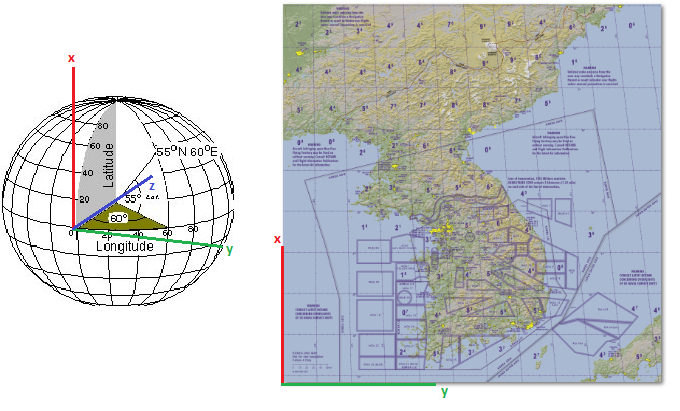
\includegraphics[width=5.5in]{Coordinates.png}
			\caption{Falcon's coordinate system.}
			\label{figure:ZZZ_Coordinates}
		\end{figure}
	\end{minipage}
\end{center}

\newpage
Given latitude and longitude, $Lat$ and $Lon$, one can essentially determine the $x$ and $y$ values in reverse of the above equations:

\begin{equation}
x= 3,359,580 \cdot \biggr( \frac{Lat - Lat_o}{Lat_{max}-Lat_{min}} \biggr)
\end{equation}
\begin{equation}
y= 3,359,580 \cdot \biggr( \frac{Lon - Lon_o}{Lon_{max}-Lon_{min}} \biggr)\cdot \biggr( \frac{cos(Lat_o)}{cos(Lat)} \biggr)
\end{equation}

\newpage
\chead{References}
\begin{thebibliography}{1}

	\bibitem{NUREG1282} {\em Safety Evaluation Report on High-Uranium Content, Low-Enriched Uranium-Zirconium Hydride Fuels for TRIGA Reactors}, NUREG-1282, Docket number 50-163, GA Technologies, August 1987.
	
	\bibitem{CpUranium} Ginnings D.C., Corruccini R.J., {\em Heat Capacities at High Temperatures of Uranium, Uranium Trichloride, and Uranium Tetrachloride}, Journal of Research of the National Bureau of Standards, Research Paper RP1831, Volume 39, October 1947.
	
	\bibitem{CpZircHydride} Douglas T.B., Victor A.C., {\em Heat Content of Zirconium and of Five Compositions of Zirconium Hydride from $0^{\circ}$ to $990^{\circ}C$}, Journal of Research of the National Bureau of Standards, Research Paper RP2878, Volume 61, July 1958.
	
\end{thebibliography}

\newpage
\chead{Appendix}
\appendix
\begin{landscape}
\section{FlightData.h}

\appendix
\begin{lstlisting}
#ifndef _FLIGHT_DATA_H
#define _FLIGHT_DATA_H


#define FLIGHTDATA_VERSION 117
// changelog:
// 110: initial BMS 4.33 version
// 111: added SysTest to LightBits3
// 112: added MCAnnounced to LightBits3
// 113: added AllLampBits2OnExceptCarapace to LightBits2 and AllLampBits3OnExceptCarapace to LightBits3
// 114: renamed WOW LightBit to ONGROUND, added "real" (AFM) WOW to LightBits3
// 115: renamed "real" WOW in MLGWOW, added NLGWOW
// 116: bitfields are now unsigned instead of signed
// 117: added ATF_Not_Engaged to LightBits3

// *** "FalconSharedMemoryArea" ***,
class FlightData 
{
public:
	// GENERAL NOTE FOR ALL LIGHTBITS:
	//
	// The lightbits contain status about whether a lamp is activated or deactivated. A *blinking* lamp
	// is always activated, even if it is in the "off" phase of the blinking! To check whether an activated
	// lamp is blinking or just "on", use the BlinkBits in FlightData2. A blinkbit does NOT alternate on/off
	// either, it will just state *if* a lamp is blinking. This construct might seem strange at 1st sight,
	// but only like this it can be guaranteed that even low-freq shared mem readers will pick up the info
	// about blinking lamps correctly. Obviously, it is up to the external program to implement the actual
	// blinking logic/freq etc.
	//
	// Summary:
	// a) The LightBit says "lamp is active (LightBit 1) or inactive (LightBit 0)".
	// b) The BlinkBit says "if the lamp is active (see LightBit 1), is it steady (BlinkBit 0)
	//    or is it blinking (BlinkBit 1)"
	// c) If a lamp has no BlinkBit, it is always assumed to be steady if active (LightBit 1).
	
	enum LightBits
    {
        MasterCaution = 0x1,  // Left eyebrow

        // Brow Lights
        TF        = 0x2,   // Left eyebrow
        OXY_BROW  = 0x4,   // repurposed for eyebrow OXY LOW (was OBS, unused)
        EQUIP_HOT = 0x8,   // Caution light; repurposed for cooling fault (was: not used)
        ONGROUND  = 0x10,  // True if on ground: this is not a lamp bit!
        ENG_FIRE  = 0x20,  // Right eyebrow; upper half of split face lamp
        CONFIG    = 0x40,  // Stores config, caution panel
        HYD       = 0x80,  // Right eyebrow; see also OIL (this lamp is not split face)
        Flcs_ABCD = 0x100, // TEST panel FLCS channel lamps; repurposed, was OIL (see HYD; that lamp is not split face)
        FLCS      = 0x200, // Right eyebrow; was called DUAL which matches block 25, 30/32 and older 40/42
        CAN       = 0x400, // Right eyebrow
        T_L_CFG   = 0x800, // Right eyebrow

        // AOA Indexers
        AOAAbove  = 0x1000,
        AOAOn     = 0x2000,
        AOABelow  = 0x4000,

        // Refuel/NWS
        RefuelRDY = 0x8000,
        RefuelAR  = 0x10000,
        RefuelDSC = 0x20000,

        // Caution Lights
        FltControlSys = 0x40000,
        LEFlaps       = 0x80000,
        EngineFault   = 0x100000,
        Overheat      = 0x200000,
        FuelLow       = 0x400000,
        Avionics      = 0x800000,
        RadarAlt      = 0x1000000,
        IFF           = 0x2000000,
        ECM           = 0x4000000,
        Hook          = 0x8000000,
        NWSFail       = 0x10000000,
        CabinPress    = 0x20000000,

        AutoPilotOn   = 0x40000000,  // TRUE if is AP on.  NB: This is not a lamp bit!
        TFR_STBY      = 0x80000000,  // MISC panel; lower half of split face TFR lamp

        // Used with the MAL/IND light code to light up "everything"
        // please update this if you add/change bits!
        AllLampBitsOn     = 0xBFFFFFEF
    };

    enum LightBits2
    {
        // Threat Warning Prime
        HandOff = 0x1,
        Launch  = 0x2,
        PriMode = 0x4,
        Naval   = 0x8,
        Unk     = 0x10,
        TgtSep  = 0x20,

		// EWS
		Go		= 0x40,		// On and operating normally
		NoGo    = 0x80,     // On but malfunction present
		Degr    = 0x100,    // Status message: AUTO DEGR
		Rdy     = 0x200,    // Status message: DISPENSE RDY
		ChaffLo = 0x400,    // Bingo chaff quantity reached
		FlareLo = 0x800,    // Bingo flare quantity reached

        // Aux Threat Warning
        AuxSrch = 0x1000,
        AuxAct  = 0x2000,
        AuxLow  = 0x4000,
        AuxPwr  = 0x8000,

        // ECM
        EcmPwr  = 0x10000,
        EcmFail = 0x20000,

        // Caution Lights
        FwdFuelLow = 0x40000,
        AftFuelLow = 0x80000,

        EPUOn      = 0x100000,  // EPU panel; run light
        JFSOn      = 0x200000,  // Eng Jet Start panel; run light

        // Caution panel
        SEC          = 0x400000,
        OXY_LOW      = 0x800000,
        PROBEHEAT    = 0x1000000,
        SEAT_ARM     = 0x2000000,
        BUC          = 0x4000000,
        FUEL_OIL_HOT = 0x8000000,
        ANTI_SKID    = 0x10000000,

        TFR_ENGAGED  = 0x20000000,  // MISC panel; upper half of split face TFR lamp
        GEARHANDLE   = 0x40000000,  // Lamp in gear handle lights on fault or gear in motion
        ENGINE       = 0x80000000,  // Lower half of right eyebrow ENG FIRE/ENGINE lamp

        // Used with the MAL/IND light code to light up "everything"
        // please update this if you add/change bits!
		AllLampBits2On = 0xFFFFF03F,
		AllLampBits2OnExceptCarapace = AllLampBits2On ^ HandOff ^ Launch ^ PriMode ^ Naval ^ Unk ^ TgtSep ^ AuxSrch ^ AuxAct ^ AuxLow ^ AuxPwr
    };

    enum LightBits3
    {
        // Elec panel
        FlcsPmg = 0x1,
        MainGen = 0x2,
        StbyGen = 0x4,
        EpuGen  = 0x8,
        EpuPmg  = 0x10,
        ToFlcs  = 0x20,
        FlcsRly = 0x40,
        BatFail = 0x80,

        // EPU panel
        Hydrazine = 0x100,
        Air       = 0x200,

        // Caution panel
        Elec_Fault = 0x400,
        Lef_Fault  = 0x800,

		OnGround	  = 0x1000,   // weight-on-wheels
        FlcsBitRun    = 0x2000,   // FLT CONTROL panel RUN light (used to be Multi-engine fire light)
        FlcsBitFail   = 0x4000,   // FLT CONTROL panel FAIL light (used to be Lock light Cue; non-F-16)
        DbuWarn       = 0x8000,   // Right eyebrow DBU ON cell; was Shoot light cue; non-F16
        NoseGearDown  = 0x10000,  // Landing gear panel; on means down and locked
        LeftGearDown  = 0x20000,  // Landing gear panel; on means down and locked
        RightGearDown = 0x40000,  // Landing gear panel; on means down and locked
		ParkBrakeOn   = 0x100000, // Parking brake engaged; NOTE: not a lamp bit
        Power_Off     = 0x200000, // Set if there is no electrical power.  NB: not a lamp bit

		// Caution panel
		cadc	= 0x400000,
		
		// Left Aux console
		SpeedBrake = 0x800000,  // True if speed brake is in anything other than stowed position

        // Threat Warning Prime - additional bits
		SysTest  = 0x1000000,

		// Master Caution WILL come up (actual lightBit has 3sec delay like in RL),
		// usable for cockpit builders with RL equipment which has a delay on its own.
		// Will be set to false again as soon as the MasterCaution bit is set.
		MCAnnounced = 0x2000000,

		//MLGWOW is only for AFM , it means WOW switches on MLG are triggered => FLCS switches to WOWPitchRockGain
		MLGWOW = 0x4000000,
		NLGWOW = 0x8000000,

		ATF_Not_Engaged = 0x10000000,
		
		// Free bits in LightBits3		
		//0x20000000,
		//0x40000000,
		//0x80000000,

		// Used with the MAL/IND light code to light up "everything"
        // please update this if you add/change bits!
		AllLampBits3On = 0x1147EFFF,
		AllLampBits3OnExceptCarapace = AllLampBits3On ^ SysTest
    };

    enum HsiBits
    {
        ToTrue        = 0x01,    // HSI_FLAG_TO_TRUE == 1, TO
        IlsWarning    = 0x02,    // HSI_FLAG_ILS_WARN
        CourseWarning = 0x04,    // HSI_FLAG_CRS_WARN
        Init          = 0x08,    // HSI_FLAG_INIT
        TotalFlags    = 0x10,    // HSI_FLAG_TOTAL_FLAGS; never set
        ADI_OFF       = 0x20,    // ADI OFF Flag
        ADI_AUX       = 0x40,    // ADI AUX Flag
        ADI_GS        = 0x80,    // ADI GS FLAG
        ADI_LOC       = 0x100,   // ADI LOC FLAG
        HSI_OFF       = 0x200,   // HSI OFF Flag
        BUP_ADI_OFF   = 0x400,   // Backup ADI Off Flag
        VVI           = 0x800,   // VVI OFF Flag
        AOA           = 0x1000,  // AOA OFF Flag
        AVTR          = 0x2000,  // AVTR Light
		OuterMarker   = 0x4000,  // MARKER beacon light for outer marker
		MiddleMarker  = 0x8000,  // MARKER beacon light for middle marker
		FromTrue      = 0x10000, // HSI_FLAG_TO_TRUE == 2, FROM

		Flying		  = 0x80000000, // true if player is attached to an aircraft (i.e. not in UI state).  NOTE: Not a lamp bit

		// Used with the MAL/IND light code to light up "everything"
        // please update this is you add/change bits!
        AllLampHsiBitsOn = 0xE000
    };

    // These are outputs from the sim
	// Note: some two-engine values removed in this version for compatibility
	// reasons.
    float x;            // Ownship North (Ft)
    float y;            // Ownship East (Ft)
    float z;            // Ownship Down (Ft) --- NOTE: use FlightData2 AAUZ for barometric altitude!
    float xDot;         // Ownship North Rate (ft/sec)
    float yDot;         // Ownship East Rate (ft/sec)
    float zDot;         // Ownship Down Rate (ft/sec)
    float alpha;        // Ownship AOA (Degrees)
    float beta;         // Ownship Beta (Degrees)
    float gamma;        // Ownship Gamma (Radians)
    float pitch;        // Ownship Pitch (Radians)
    float roll;         // Ownship Pitch (Radians)
    float yaw;          // Ownship Pitch (Radians)
    float mach;         // Ownship Mach number
    float kias;         // Ownship Indicated Airspeed (Knots)
    float vt;           // Ownship True Airspeed (Ft/Sec)
    float gs;           // Ownship Normal Gs
    float windOffset;   // Wind delta to FPM (Radians)
    float nozzlePos;    // Ownship engine nozzle percent open (0-100)
	//float nozzlePos2;   // MOVED TO FlightData2! Ownship engine nozzle2 percent open (0-100) 
    float internalFuel; // Ownship internal fuel (Lbs)
    float externalFuel; // Ownship external fuel (Lbs)
    float fuelFlow;     // Ownship fuel flow (Lbs/Hour)
    float rpm;          // Ownship engine rpm (Percent 0-103)
	//float rpm2;         // MOVED TO FlightData2! Ownship engine rpm2 (Percent 0-103)
    float ftit;         // Ownship Forward Turbine Inlet Temp (Degrees C)
	//float ftit2;        // MOVED TO FlightData2! Ownship Forward Turbine Inlet Temp2 (Degrees C)
    float gearPos;      // Ownship Gear position 0 = up, 1 = down;
    float speedBrake;   // Ownship speed brake position 0 = closed, 1 = 60 Degrees open
    float epuFuel;      // Ownship EPU fuel (Percent 0-100)
    float oilPressure;  // Ownship Oil Pressure (Percent 0-100)
	//float oilPressure2; // MOVED TO FlightData2! Ownship Oil Pressure2 (Percent 0-100)
    unsigned int   lightBits;    // Cockpit Indicator Lights, one bit per bulb. See enum

    // These are inputs. Use them carefully
	// NB: these do not work when TrackIR device is enabled
	// NB2: launch falcon with the '-head' command line parameter to activate !
    float headPitch;    // Head pitch offset from design eye (radians)
    float headRoll;     // Head roll offset from design eye (radians)
    float headYaw;      // Head yaw offset from design eye (radians)

    // new lights
    unsigned int   lightBits2;   // Cockpit Indicator Lights, one bit per bulb. See enum
    unsigned int   lightBits3;   // Cockpit Indicator Lights, one bit per bulb. See enum

    // chaff/flare
    float ChaffCount;   // Number of Chaff left
    float FlareCount;   // Number of Flare left

    // landing gear
    float NoseGearPos;  // Position of the nose landinggear; caution: full down values defined in dat files
    float LeftGearPos;  // Position of the left landinggear; caution: full down values defined in dat files
    float RightGearPos; // Position of the right landinggear; caution: full down values defined in dat files

    // ADI values
    float AdiIlsHorPos; // Position of horizontal ILS bar
    float AdiIlsVerPos; // Position of vertical ILS bar

    // HSI states
    int courseState;    // HSI_STA_CRS_STATE
    int headingState;   // HSI_STA_HDG_STATE
    int totalStates;    // HSI_STA_TOTAL_STATES; never set

    // HSI values
    float courseDeviation;     // HSI_VAL_CRS_DEVIATION
    float desiredCourse;       // HSI_VAL_DESIRED_CRS
    float distanceToBeacon;    // HSI_VAL_DISTANCE_TO_BEACON
    float bearingToBeacon;     // HSI_VAL_BEARING_TO_BEACON
    float currentHeading;      // HSI_VAL_CURRENT_HEADING
    float desiredHeading;      // HSI_VAL_DESIRED_HEADING
    float deviationLimit;      // HSI_VAL_DEV_LIMIT
    float halfDeviationLimit;  // HSI_VAL_HALF_DEV_LIMIT
    float localizerCourse;     // HSI_VAL_LOCALIZER_CRS
    float airbaseX;            // HSI_VAL_AIRBASE_X
    float airbaseY;            // HSI_VAL_AIRBASE_Y
    float totalValues;         // HSI_VAL_TOTAL_VALUES; never set

    float TrimPitch;  // Value of trim in pitch axis, -0.5 to +0.5
    float TrimRoll;   // Value of trim in roll axis, -0.5 to +0.5
    float TrimYaw;    // Value of trim in yaw axis, -0.5 to +0.5

    // HSI flags
    unsigned int hsiBits;      // HSI flags

    //DED Lines
    char DEDLines[5][26];  //25 usable chars
    char Invert[5][26];    //25 usable chars

    //PFL Lines
    char PFLLines[5][26];  //25 usable chars
    char PFLInvert[5][26]; //25 usable chars

    //TacanChannel
    int UFCTChan, AUXTChan;

    // RWR
    int           RwrObjectCount;
    int           RWRsymbol[40];
    float         bearing[40];
    unsigned long missileActivity[40];
    unsigned long missileLaunch[40];
    unsigned long selected[40];
    float         lethality[40];
	unsigned long newDetection[40];

    //fuel values
    float fwd, aft, total;

    void SetLightBit (unsigned int newBit) {lightBits |= newBit;};
	void ClearLightBit(unsigned int newBit) { lightBits &= ~newBit; };
	bool IsSet(unsigned int newBit) { return ((lightBits & newBit) ? true : false); };

	void SetLightBit2(unsigned int newBit) { lightBits2 |= newBit; };
	void ClearLightBit2(unsigned int newBit) { lightBits2 &= ~newBit; };
	bool IsSet2(unsigned int newBit) { return ((lightBits2 & newBit) ? true : false); };

	void SetLightBit3(unsigned int newBit) { lightBits3 |= newBit; };
	void ClearLightBit3(unsigned int newBit) { lightBits3 &= ~newBit; };
	bool IsSet3(unsigned int newBit) { return ((lightBits3 & newBit) ? true : false); };

	void SetHsiBit(unsigned int newBit) { hsiBits |= newBit; };
	void ClearHsiBit(unsigned int newBit) { hsiBits &= ~newBit; };
	bool IsSetHsi(unsigned int newBit) { return ((hsiBits & newBit) ? true : false); };

    int VersionNum;    // Version of FlightData mem area

    // New values added here for header file compatibility but not implemented
    // in this version of the code at present.
    float headX;       // Head X offset from design eye (feet)
    float headY;       // Head Y offset from design eye (feet)
    float headZ;       // Head Z offset from design eye (feet)

    int MainPower;     // Main Power switch state, 0=down, 1=middle, 2=up
};


// OSB capture for MFD button labeling

#define OSB_STRING_LENGTH 8  // currently strings appear to be max 7 printing chars

typedef struct {
	char line1[OSB_STRING_LENGTH];
	char line2[OSB_STRING_LENGTH];
	bool inverted;
} OsbLabel;


// *** "FalconSharedOsbMemoryArea" ***
class OSBData
{
public:
	OsbLabel leftMFD[20];
	OsbLabel rightMFD[20];
};


#define FLIGHTDATA2_VERSION 9
// changelog:
// 1: initial BMS 4.33 version
// 2: added AltCalReading, altBits, BupUhfPreset, powerBits, blinkBits, cmdsMode
// 3: added VersionNum, hydPressureA/B, cabinAlt, BupUhfFreq, currentTime, vehicleACD
// 4: added fuelflow2
// 5: added RwrInfo, lefPos, tefPos
// 6: added vtolPos
// 7: bit fields are now unsigned instead of signed
// 8: increased RwrInfo size to 512
// 9: added human pilot names and their status in a session

// do NOT change these w/o crosschecking the BMS code
#define RWRINFO_SIZE 512
#define CALLSIGN_LEN 12
#define MAX_CALLSIGNS 32

// *** "FalconSharedMemoryArea2" ***
class FlightData2
{
public:

	// TACAN
	enum TacanSources
	{
		UFC = 0,
		AUX = 1,
		NUMBER_OF_SOURCES = 2,
	};
	enum TacanBits
	{
		band = 0x01,   // true in this bit position if band is X
		mode = 0x02,   // true in this bit position if domain is air to air
	};

	// ALTIMETER
	enum AltBits
	{
		CalType  = 0x01,	// true if calibration in inches of Mercury (Hg), false if in hectoPascal (hPa)
		PneuFlag = 0x02,	// true if PNEU flag is visible
	};

	// POWER
	enum PowerBits
	{
		BusPowerBattery      = 0x01,	// true if at least the battery bus is powered
		BusPowerEmergency    = 0x02,	// true if at least the emergency bus is powered
		BusPowerEssential    = 0x04,	// true if at least the essential bus is powered
		BusPowerNonEssential = 0x08,	// true if at least the non-essential bus is powered
		MainGenerator        = 0x10,	// true if the main generator is online
		StandbyGenerator     = 0x20,	// true if the standby generator is online
		JetFuelStarter       = 0x40,	// true if JFS is running, can be used for magswitch
	};

	// BLINKING LIGHTS - only indicating *IF* a lamp is blinking, not implementing the actual on/off/blinking pattern logic!
	enum BlinkBits
	{
		// currently working
		OuterMarker  = 0x01,	// defined in HsiBits    - slow flashing for outer marker
		MiddleMarker = 0x02,	// defined in HsiBits    - fast flashing for middle marker
		PROBEHEAT    = 0x04,	// defined in LightBits2 - probeheat system is tested
		AuxSrch      = 0x08,	// defined in LightBits2 - search function in NOT activated and a search radar is painting ownship
		Launch       = 0x10,	// defined in LightBits2 - missile is fired at ownship
		PriMode      = 0x20,	// defined in LightBits2 - priority mode is enabled but more than 5 threat emitters are detected
		Unk          = 0x40,	// defined in LightBits2 - unknown is not active but EWS detects unknown radar

		// not working yet, defined for future use
		Elec_Fault   = 0x80,	// defined in LightBits3 - non-resetting fault
		OXY_BROW     = 0x100,	// defined in LightBits  - monitor fault during Obogs
		EPUOn        = 0x200,	// defined in LightBits3 - abnormal EPU operation
		JFSOn_Slow   = 0x400,	// defined in LightBits3 - slow blinking: non-critical failure
		JFSOn_Fast   = 0x800,	// defined in LightBits3 - fast blinking: critical failure
	};

	// CMDS mode state
	enum CmdsModes
	{
		CmdsOFF  = 0,
		CmdsSTBY = 1,
		CmdsMAN  = 2,
		CmdsSEMI = 3,
		CmdsAUTO = 4,
		CmdsBYP  = 5,
	};

	// HSI/eHSI mode state
	enum NavModes 
	{
		ILS_TACAN   = 0,
		TACAN       = 1, 
		NAV         = 2,
		ILS_NAV     = 3,
	};

	// human pilot state
	enum FlyStates
	{
		IN_UI   = 0, // UI      - in the UI
		LOADING = 1, // UI>3D   - loading the sim data
		WAITING = 2, // UI>3D   - waiting for other players
		FLYING  = 3, // 3D      - flying
		DEAD    = 4, // 3D>Dead - dead, waiting to respawn
		UNKNOWN = 5, // ???
	};

	// VERSION 1
	float nozzlePos2;       // Ownship engine nozzle2 percent open (0-100)
	float rpm2;             // Ownship engine rpm2 (Percent 0-103)
	float ftit2;            // Ownship Forward Turbine Inlet Temp2 (Degrees C)
	float oilPressure2;     // Ownship Oil Pressure2 (Percent 0-100)
	unsigned char navMode;  // current mode selected for HSI/eHSI, see NavModes enum for details
	float AAUZ;             // Ownship barometric altitude given by AAU (depends on calibration)
	char tacanInfo[NUMBER_OF_SOURCES]; // Tacan band/mode settings for UFC and AUX COMM

	// VERSION 2 / 7
	int AltCalReading;	// barometric altitude calibration (depends on CalType)
	unsigned int altBits;		// various altimeter bits, see AltBits enum for details
	unsigned int powerBits;		// Ownship power bus / generator states, see PowerBits enum for details
	unsigned int blinkBits;		// Cockpit indicator lights blink status, see BlinkBits enum for details
						// NOTE: these bits indicate only *if* a lamp is blinking, in addition to the
						// existing on/off bits. It's up to the external program to implement the
						// *actual* blinking.
	int cmdsMode;		// Ownship CMDS mode state, see CmdsModes enum for details
	int BupUhfPreset;	// BUP UHF channel preset

	// VERSION 3
	int BupUhfFreq;		// BUP UHF channel frequency
	float cabinAlt;		// Ownship cabin altitude
	float hydPressureA;	// Ownship Hydraulic Pressure A
	float hydPressureB;	// Ownship Hydraulic Pressure B
	int currentTime;	// Current time in seconds (max 60 * 60 * 24)
	short vehicleACD;	// Ownship ACD index number, i.e. which aircraft type are we flying.
	int VersionNum;		// Version of FlightData2 mem area

	// VERSION 4
	float fuelFlow2;    // Ownship fuel flow2 (Lbs/Hour)

	// VERSION 5 / 8
	char RwrInfo[RWRINFO_SIZE]; // New RWR Info
	float lefPos;               // Ownship LEF position
	float tefPos;               // Ownship TEF position

	// VERSION 6
	float vtolPos;      // Ownship VTOL exhaust angle

	// VERSION 9
	char pilotsOnline;                                // Number of pilots in an MP session
	char pilotsCallsign[MAX_CALLSIGNS][CALLSIGN_LEN]; // List of pilots callsign connected to an MP session
	char pilotsStatus[MAX_CALLSIGNS];                 // Status of the MP pilots, see enum FlyStates

	// TACAN
	// setters for internal use only
	void SetUfcTacanToAA(bool t) { if (t) { tacanInfo[UFC] |= mode; } else { tacanInfo[UFC] &= ~mode; } }
	void SetAuxTacanToAA(bool t) { if (t) { tacanInfo[AUX] |= mode; } else { tacanInfo[AUX] &= ~mode; } }
	void SetUfcTacanToX(bool t)  { if (t) { tacanInfo[UFC] |= band; } else { tacanInfo[UFC] &= ~band; } }
	void SetAuxTacanToX(bool t)  { if (t) { tacanInfo[AUX] |= band; } else { tacanInfo[AUX] &= ~band; } }

	// getters for external reader programs
	bool UfcTacanIsAA(void) {return ((tacanInfo[UFC] & mode) ? true : false); }
	bool AuxTacanIsAA(void) {return ((tacanInfo[AUX] & mode) ? true : false); }
	bool UfcTacanIsX(void)  {return ((tacanInfo[UFC] & band) ? true : false); }
	bool AuxTacanIsX(void)  {return ((tacanInfo[AUX] & band) ? true : false); }

	// ALTIMETER
	void SetAltBit(unsigned int newBit) { altBits |= newBit; };
	void ClearAltBit(unsigned int newBit) { altBits &= ~newBit; };
	bool IsSetAlt(unsigned int newBit) { return ((altBits & newBit) ? true : false); };

	// POWER
	void SetPowerBit(unsigned int newBit) { powerBits |= newBit; };
	void ClearPowerBit(unsigned int newBit) { powerBits &= ~newBit; };
	bool IsSetPower(unsigned int newBit) { return ((powerBits & newBit) ? true : false); };

    // BLINKING LIGHTS
	void SetBlinkBit(unsigned int newBit) { blinkBits |= newBit; };
	void ClearBlinkBit(unsigned int newBit) { blinkBits &= ~newBit; };
	bool IsSetBlink(unsigned int newBit) { return ((blinkBits & newBit) ? true : false); };

	// CMDS mode state
	void SetCmdsMode(int newMode) {cmdsMode = newMode;};
	int  GetCmdsMode(void) {return cmdsMode;};

	// HSI/eHSI mode state
	void SetNavMode(int newMode) {navMode = newMode;};
	int  GetNavMode(void) {return navMode;};
};


extern OSBData cockpitOSBData;         // "FalconSharedOsbMemoryArea"
extern FlightData cockpitFlightData;   // "FalconSharedMemoryArea"
extern FlightData2 cockpitFlightData2; // "FalconSharedMemoryArea2"

#endif

\end{lstlisting}


\end{landscape}



\end{document}